\documentclass[tikz,border=2pt]{standalone}
\usepackage{unicode-math}
\setmainfont[
  Path=publication/fonts/,
  UprightFont=source-serif-4-latin-400-normal.ttf,
  ItalicFont=source-serif-4-latin-400-italic.ttf,
  BoldFont=source-serif-4-latin-600-normal.ttf,
  BoldItalicFont=source-serif-4-latin-600-italic.ttf
]{Source Serif 4}
\setmathfont[Path=/System/Library/Fonts/Supplemental/]{STIXTwoMath.otf}
\usepackage{tikz}
\usetikzlibrary{arrows.meta,backgrounds,calc,decorations.pathreplacing,fit,matrix,positioning}
\definecolor{BookInk}{HTML}{18232D}
\definecolor{BookBlue}{HTML}{315F78}
\definecolor{BookRed}{HTML}{98452F}
\definecolor{BookGreen}{HTML}{3F6659}
\definecolor{BookMuted}{HTML}{66727A}
\definecolor{BookRule}{HTML}{AEB7BC}
\tikzset{
  book/node/.style={
    draw=BookInk, line width=.55pt, fill=white,
    minimum height=9mm, inner xsep=5pt, inner ysep=4pt,
    font=\footnotesize, align=center
  },
  book/primary/.style={book/node, draw=BookBlue},
  book/decision/.style={book/node, draw=BookRed},
  book/verified/.style={book/node, draw=BookGreen},
  book/arrow/.style={
    -{Stealth[length=2mm,width=1.35mm]}, line width=.55pt, draw=BookInk
  },
  book/quietarrow/.style={
    -{Stealth[length=2mm,width=1.35mm]}, line width=.45pt, draw=BookRule
  },
  book/feedback/.style={
    -{Stealth[length=2mm,width=1.35mm]}, line width=.5pt,
    draw=BookRed, dashed
  },
  book/note/.style={font=\scriptsize, text=BookMuted, align=center}
}

\begin{document}
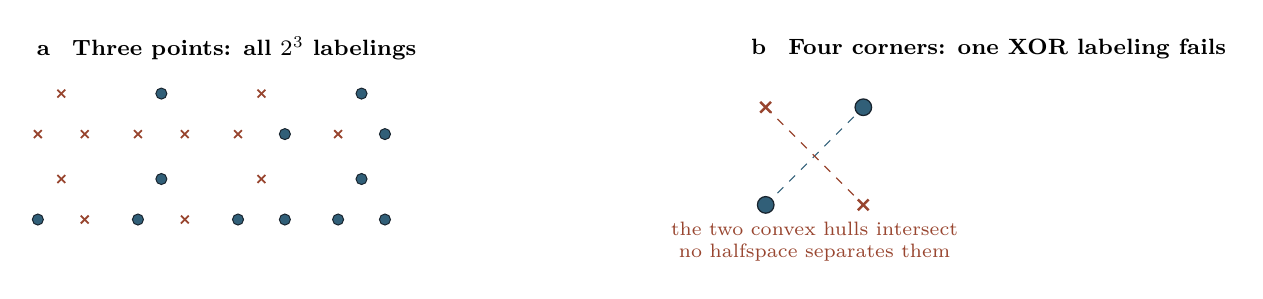
\begin{tikzpicture}[x=.62cm,y=.62cm]
  \node[font=\footnotesize\bfseries,anchor=west] at (0,4.5)
    {a\quad Three points: all $2^3$ labelings};
  \newcommand{\vcp}[3]{%
    \ifnum#3=1
      \filldraw[fill=BookBlue,draw=BookInk,line width=.35pt] (#1,#2) circle (2pt);
    \else
      \draw[BookRed,line width=.65pt] (#1-.08,#2-.08)--(#1+.08,#2+.08);
      \draw[BookRed,line width=.65pt] (#1-.08,#2+.08)--(#1+.08,#2-.08);
    \fi}
  \newcommand{\vctri}[5]{%
    \vcp{#1-.48}{#2-.35}{#3}
    \vcp{#1+.48}{#2-.35}{#4}
    \vcp{#1}{#2+.48}{#5}}
  \vctri{.7}{3.1}{0}{0}{0}
  \vctri{2.75}{3.1}{0}{0}{1}
  \vctri{4.8}{3.1}{0}{1}{0}
  \vctri{6.85}{3.1}{0}{1}{1}
  \vctri{.7}{1.35}{1}{0}{0}
  \vctri{2.75}{1.35}{1}{0}{1}
  \vctri{4.8}{1.35}{1}{1}{0}
  \vctri{6.85}{1.35}{1}{1}{1}
  \begin{scope}[xshift=10cm]
    \node[font=\footnotesize\bfseries,anchor=west] at (-1.5,4.5)
      {b\quad Four corners: one XOR labeling fails};
    \draw[BookBlue,dashed] (-1,1.3)--(1,3.3);
    \draw[BookRed,dashed] (-1,3.3)--(1,1.3);
    \foreach \x/\y in {-1/-1,1/1}{
      \filldraw[fill=BookBlue,draw=BookInk,line width=.45pt] (\x,\y+2.3) circle (3pt);
    }
    \foreach \x/\y in {-1/1,1/-1}{
      \draw[BookRed,line width=.9pt] (\x-.11,\y+2.3-.11)--(\x+.11,\y+2.3+.11);
      \draw[BookRed,line width=.9pt] (\x-.11,\y+2.3+.11)--(\x+.11,\y+2.3-.11);
    }
    \node[book/note,text=BookRed,align=center] at (0,.55)
      {the two convex hulls intersect\\no halfspace separates them};
  \end{scope}
\end{tikzpicture}
\end{document}
